
\documentclass[spanish]{article}
\usepackage{babel}
\usepackage{pdflscape}
\usepackage{tikz}
\usepackage{float}
\usepackage[utf8]{inputenc}
\usepackage{graphicx}
\restylefloat{table}
\begin{document}
\begin{titlepage}

\centering
	\vspace{1cm}
	{\scshape\LARGE Instituto Politécnico Nacional \par}
	\vspace{0.7cm}
	{\scshape\Large Escuela Superior de Cómputo\par}
	\vspace{1.5cm}
	{\huge\bfseries Conversión AFN-AFD de automata que reconoce cadenas con terminación web o ebay\par}
	\vspace{2cm}
	{\Large\itshape Mercado Rogel Martin Isauro\par}
	\vspace{0.7cm}
	{\large 2014090449\par}
	\vspace{0.7cm}
	{\large Teoría computacional\par}
	\vspace{0.7cm}
	{\large 2CV1\par}
	\vfill
	%supervised by\par
	%Dr.~Mark \textsc{Brown}

	\vfill

% Bottom of the page
	{\large \today\par}
\end{titlepage}
\section{Introducción}
Se pide convertir  el siguiente Autómata finito no determinista en determinista.\\
El automata tiene el siguiente diagrama de estados:\\
% \includegraphics[width=0.7\textwidth]{diagrama.jpeg}\\ %

\begin{center}
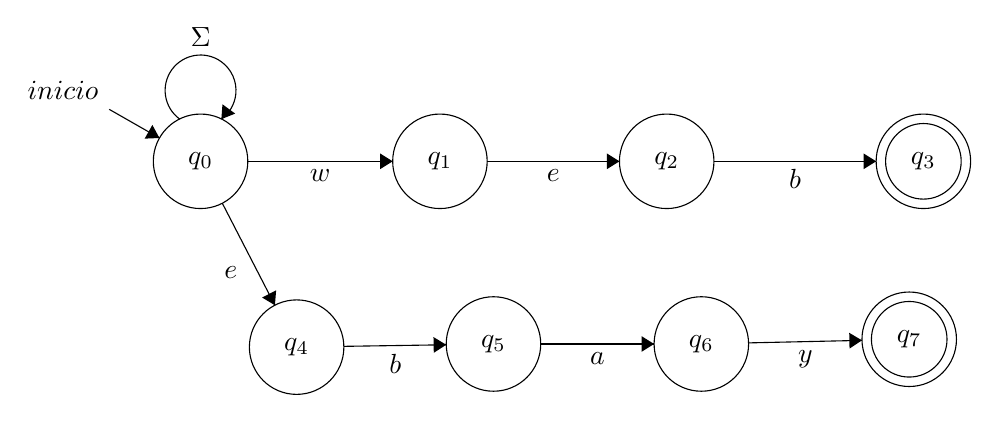
\begin{tikzpicture}[scale=0.2]
\tikzstyle{every node}+=[inner sep=0pt]
\draw [black] (29.9,-12.5) circle (3);
\draw (29.9,-12.5) node {$q_1$};
\draw [black] (14.7,-12.5) circle (3);
\draw (14.7,-12.5) node {$q_0$};
\draw [black] (44.3,-12.5) circle (3);
\draw (44.3,-12.5) node {$q_2$};
\draw [black] (60.6,-12.5) circle (3);
\draw (60.6,-12.5) node {$q_3$};
\draw [black] (60.6,-12.5) circle (2.4);
\draw [black] (20.8,-24.3) circle (3);
\draw (20.8,-24.3) node {$q_4$};
\draw [black] (33.3,-24.1) circle (3);
\draw (33.3,-24.1) node {$q_5$};
\draw [black] (46.5,-24.1) circle (3);
\draw (46.5,-24.1) node {$q_6$};
\draw [black] (59.7,-23.8) circle (3);
\draw (59.7,-23.8) node {$q_7$};
\draw [black] (59.7,-23.8) circle (2.4);
\draw [black] (8.9,-9.2) -- (12.09,-11.02);
\draw (8.24,-7.98) node [left] {$inicio$};
\fill [black] (12.09,-11.02) -- (11.64,-10.19) -- (11.15,-11.06);
\draw [black] (13.377,-9.82) arc (234:-54:2.25);
\draw (14.7,-5.25) node [above] {$\Sigma$};
\fill [black] (16.02,-9.82) -- (16.9,-9.47) -- (16.09,-8.88);
\draw [black] (17.7,-12.5) -- (26.9,-12.5);
\fill [black] (26.9,-12.5) -- (26.1,-12) -- (26.1,-13);
\draw (22.3,-13) node [below] {$w$};
\draw [black] (32.9,-12.5) -- (41.3,-12.5);
\fill [black] (41.3,-12.5) -- (40.5,-12) -- (40.5,-13);
\draw (37.1,-13) node [below] {$e$};
\draw [black] (47.3,-12.5) -- (57.6,-12.5);
\fill [black] (57.6,-12.5) -- (56.8,-12) -- (56.8,-13);
\draw (52.45,-13) node [below] {$b$};
\draw [black] (16.08,-15.16) -- (19.42,-21.64);
\fill [black] (19.42,-21.64) -- (19.5,-20.69) -- (18.61,-21.15);
\draw (17.06,-19.54) node [left] {$e$};
\draw [black] (23.8,-24.25) -- (30.3,-24.15);
\fill [black] (30.3,-24.15) -- (29.49,-23.66) -- (29.51,-24.66);
\draw (27.06,-24.72) node [below] {$b$};
\draw [black] (36.3,-24.1) -- (43.5,-24.1);
\fill [black] (43.5,-24.1) -- (42.7,-23.6) -- (42.7,-24.6);
\draw (39.9,-24.6) node [below] {$a$};
\draw [black] (49.5,-24.03) -- (56.7,-23.87);
\fill [black] (56.7,-23.87) -- (55.89,-23.39) -- (55.91,-24.39);
\draw (53.11,-24.47) node [below] {$y$};
\end{tikzpicture}
\end{center}

Como se puede ver el AFN reconoce aquellas cadenas que terminan en web o ebay\\
\section{Desarrollo}
Primero se nota que el AFN, digamos N, está compuesto por:
\begin{center}
$ N = (Q,\Sigma,F,q_{0},\Delta) $
\begin{itemize}
\item{ 
$ Q = \left\{ q_{0},q_{1},q_{2},q_{3},q_{4},q_{5},q_{6},q_{7} \right\} $ el conjunto de estados del autómata
}

\item{
$ \Sigma $ el conjunto de letras del alfabeto inglés 
}

\item{
$ F = \left\{ q_{3},q_{7} \right\} $ conjunto de estados de aceptación
}
\item{
$ q_{0} $ como estado inicial
}
\item{
$ \Delta $ la relación de transición para el AFN
}

\end{itemize}
\end{center}  

Ahora, se puede ver como la cardinalidad del conjunto de estados es $ \vert Q \vert = 8 $ ,
para la conversión a su AFD, digamos D, este será: 

\begin{center}
$ D = (Q \prime ,\Sigma,F \prime,\{ q_{0} \} ,\delta) $
\begin{itemize}
\item{ 
$ Q \prime = \mathcal{P}(Q) $ el conjunto de estados del autómata determinista será el conjunto potencia del conjunto de estados del AFN
}

\item{
$ \Sigma $ el alfabeto es el mismo
}

\item{
$ F \prime = \{ q \mid q \in Q \prime \cap F \neq \emptyset \} $ conjunto de estados de aceptación tales que existe un q que pertence a algun subconjunto de F prima y su intersección con F no es vacía
}
\item{
$ \{ q_{0} \} $ como estado inicial
}
\item{
$ \delta $ la función de transición para el AFD tiene la siguiente tabla:\hfill \break

\begin{table}[H]
\begin{tabular}{l|llllll}
$\delta$ & $\Sigma_{webay}$ & w & e & b & a & y  \\ \hline
$\rightarrow \{q_{0}\}$   &   $\{q_{0}\} $    & $\{q_{0},q_{1}\}$  & $\{q_{0},q_{4}\}$   & $\{q_{0}\} $   & $\{q_{0}\} $   & $\{q_{0}\} $ \\
$\{q_{0},q_{1}\}$  &   $\{q_{0}\} $    & $\{q_{0},q_{1}\}$  & $\{q_{0},q_{2},q_{4}\}$  & $\{q_{0}\} $  &  $\{q_{0}\} $ &  $\{q_{0}\} $ \\
$\{q_{0},q_{2},q_{4}\}$    &   $\{q_{0}\} $    & $\{q_{0},q_{1}\}$ & $\{q_{0},q_{4}\}$  & $ \{q_{0},q_{3},q_{5}\}$  &  $\{q_{0}\} $ &  $\{q_{0}\} $  \\
$* \{q_{0},q_{3},q_{5}\}$    &   $\{q_{0}\} $    & $\{q_{0},q_{1}\}$  & $\{q_{0},q_{4}\}$  & $\{q_{0}\}$  &  $\{q_{0},q_{6}\}$  &  $\{q_{0}\} $  \\
$\{q_{0},q_{6}\}$    &   $\{q_{0}\} $    & $\{q_{0},q_{1}\}$ & $\{q_{0},q_{4}\}$  & $\{q_{0}\}$  &  $\{q_{0}\} $ &  $ \{q_{0},q_{7}\}$  \\
$* \{q_{0},q_{7}\}$   &   $\{q_{0}\} $    & $\{q_{0},q_{1}\}$  & $\{q_{0},q_{4}\}$  & $\{q_{0}\} $  &  $\{q_{0}\} $ &  $\{q_{0}\} $  \\
$\{q_{0},q_{4}\}$    &   $\{q_{0}\} $    & $\{q_{0},q_{1}\}$  & $\{q_{0},q_{4}\}$   & $\{q_{0},q_{5}\}$  & $\{q_{0}\} $  & $\{q_{0}\} $    \\ 
$\{q_{0},q_{5}\}$ &   $\{q_{0}\} $    & $\{q_{0},q_{1}\}$  & $\{q_{0},q_{4}\}$ & $\{q_{0}\}$ &  $\{q_{0},q_{6}\}$ & $\{q_{0}\}$
\end{tabular}
\end{table}
Siendo $\Sigma_{webay} = \Sigma \setminus \{ w, e, b, a, y, \} $ , es decir, el alfabeto sin las letras w,e,b,a,y en él.
}
\end{itemize}
\end{center}  
Se puede ver que en este caso Q prima tiene una cardinalidad $ \vert Q \prime \vert  = 2^{\vert Q \vert} = 2^8 = 256 $ estados, algunos de ellos no se pueden alcanzar desde el estado inicial por ello en la tabla solo se ponen los estados relevantes o alcanzables. 


Tomaremos en cuenta las siguientes consideraciones para simplificar el diagrama y la tabla de estados:\\ 
\begin{itemize}

\item{El alfabeto $\Sigma$ sin algunos caracteres en él, por ejemplo w,e se pondrá 
$\Sigma \setminus \{ w, e \} $ , es decir, será alfabeto sin las letras w,e en él, y así para diversos casos.}

\item{Se reetiquetarán los subconjuntos con las siguientes letras:\\
$A \rightarrow \{ q_{0} \} $ \\
$B \rightarrow \{q_{0},q_{1}\}$ \\
$C \rightarrow \{q_{0},q_{2},q_{4}\}$ \\
$D \rightarrow \{q_{0},q_{3},q_{5}\}$ \\
$E \rightarrow \{q_{0},q_{6}\}$ \\
$F \rightarrow  \{q_{0},q_{7}\}$ \\
$G \rightarrow \{q_{0},q_{4}\}$ \\
$H \rightarrow \{q_{0},q_{5}\}$ \\
De tal manera que el AFD tendrá esta notación en sus nodos}

\item{
La nueva tabla con esta notación es:\hfill \break

\begin{table}[H]
\begin{tabular}{l|llllll}
$\delta$ & $\Sigma_{webay}$ & w & e & b & a & y  \\ \hline
$\rightarrow A$   &   $A $    & $B$  & $G$   & $A $   & $A $   & $A $ \\
$B$  &   $A $    & $B$  & $C$  & $A $  &  $A $ &  $A $ \\
$C$    &   $A $    & $B$ & $G$  & $ D$  &  $A $ &  $A $  \\
$* D$    &   $A $    & $B$  & $G$  & $A$  &  $E$  &  $A $  \\
$E$    &   $A $    & $B$ & $G$  & $A$  &  $A$ &  $ F$  \\
$* F$   &   $A $    & $B$  & $G$  & $A$  &  $A $ &  $A $  \\
$G$    &   $A $    & $B$  & $G$   & $H$  & $A $  & $A $    \\ 
$H$ &   $A $    & $B$  & $G$ & $A$ &  $E$ & $A$
\end{tabular}
\end{table}

}

\end{itemize}

El diagrama de estados del AFD ya convertido es:\\
\begin{landscape}
\begin{center}
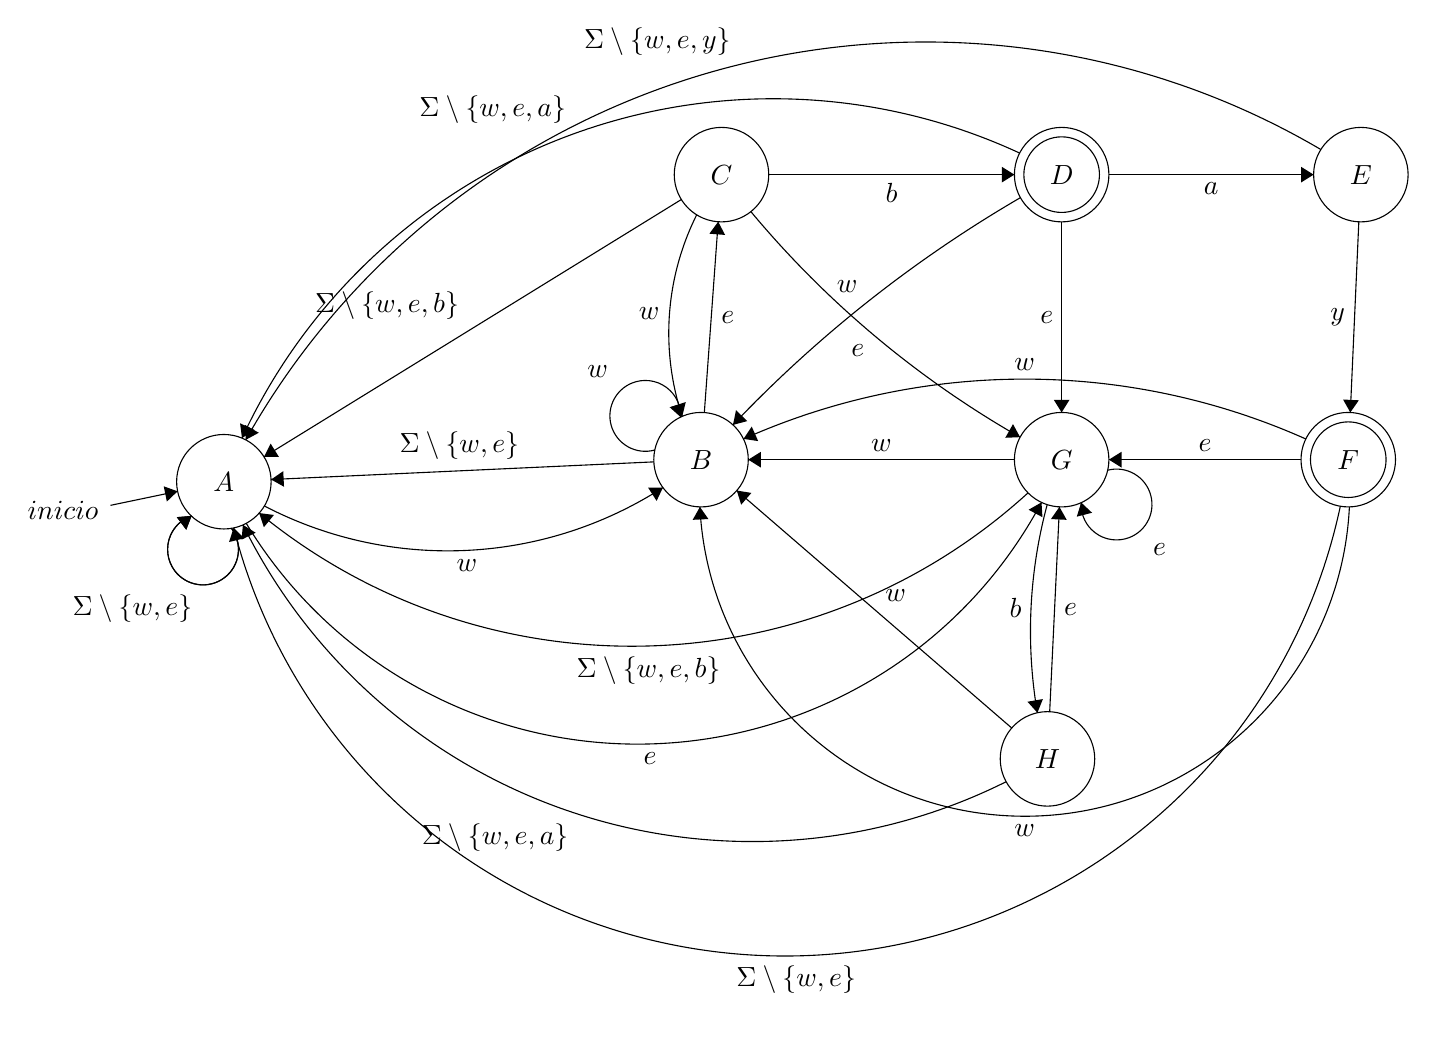
\begin{tikzpicture}[scale=0.2]
\tikzstyle{every node}+=[inner sep=0pt]
\draw [black] (0.7,-28.3) circle (3);
\draw (0.7,-28.3) node {$A$};
\draw [black] (31,-26.9) circle (3);
\draw (31,-26.9) node {$B$};
\draw [black] (32.3,-8.8) circle (3);
\draw (32.3,-8.8) node {$C$};
\draw [black] (53.9,-8.8) circle (3);
\draw (53.9,-8.8) node {$D$};
\draw [black] (53.9,-8.8) circle (2.4);
\draw [black] (72.9,-8.8) circle (3);
\draw (72.9,-8.8) node {$E$};
\draw [black] (53.9,-26.9) circle (3);
\draw (53.9,-26.9) node {$G$};
\draw [black] (72.1,-26.9) circle (3);
\draw (72.1,-26.9) node {$F$};
\draw [black] (72.1,-26.9) circle (2.4);
\draw [black] (53,-45.9) circle (3);
\draw (53,-45.9) node {$H$};
\draw [black] (-6.5,-29.8) -- (-2.24,-28.91);
\draw (-7.24,-30.14) node [left] {$inicio$};
\fill [black] (-2.24,-28.91) -- (-3.12,-28.59) -- (-2.92,-29.56);
\draw [black] (28.58,-28.671) arc (-57.21247:-117.49663:25.227);
\fill [black] (28.58,-28.67) -- (27.64,-28.68) -- (28.18,-29.52);
\draw (16.14,-33.22) node [below] {$w$};
\draw [black] (28.076,-26.283) arc (285.82111:-2.17889:2.25);
\draw (25.13,-21.31) node [left] {$w$};
\fill [black] (29.71,-24.2) -- (29.97,-23.3) -- (29.01,-23.57);
\draw [black] (29.75,-10.38) -- (3.25,-26.72);
\fill [black] (3.25,-26.72) -- (4.2,-26.73) -- (3.67,-25.88);
\draw (11.06,-18.05) node [above] {$\Sigma \setminus \{w,e,b\}$};
\draw [black] (29.806,-24.152) arc (-161.63668:-206.57954:16.791);
\fill [black] (29.81,-24.15) -- (30.03,-23.24) -- (29.08,-23.55);
\draw (28.39,-17.61) node [left] {$w$};
\draw [black] (35.3,-8.8) -- (50.9,-8.8);
\fill [black] (50.9,-8.8) -- (50.1,-8.3) -- (50.1,-9.3);
\draw (43.1,-9.3) node [below] {$b$};
\draw [black] (1.85,-25.53) arc (155.13569:65.12426:37.186);
\fill [black] (1.85,-25.53) -- (2.64,-25.01) -- (1.73,-24.59);
\draw (17.77,-5.61) node [above] {$\Sigma \setminus \{w,e,a\}$};
\draw [black] (56.9,-8.8) -- (69.9,-8.8);
\fill [black] (69.9,-8.8) -- (69.1,-8.3) -- (69.1,-9.3);
\draw (63.4,-9.3) node [below] {$a$};
\draw [black] (2.089,-25.642) arc (150.66937:59.55866:49.527);
\fill [black] (2.09,-25.64) -- (2.92,-25.19) -- (2.05,-24.7);
\draw (28.22,-1.26) node [above] {$\Sigma \setminus \{w,e,y\}$};
\draw [black] (1.176,-31.25) arc (36.89727:-251.10273:2.25);
\draw (-5.11,-35.46) node [below] {$\Sigma \setminus \{w,e\}$};
\fill [black] (-1.35,-30.47) -- (-2.29,-30.55) -- (-1.69,-31.35);
\draw [black] (1.176,-31.25) arc (36.89727:-251.10273:2.25);
\fill [black] (-1.35,-30.47) -- (-2.29,-30.55) -- (-1.69,-31.35);
\draw [black] (52.622,-29.613) arc (-28.1864:-148.79873:29.079);
\fill [black] (52.62,-29.61) -- (51.8,-30.08) -- (52.68,-30.55);
\draw (27.77,-45.47) node [below] {$e$};
\draw [black] (56.812,-27.571) arc (104.75913:-183.24087:2.25);
\draw (59.68,-32.6) node [right] {$e$};
\fill [black] (55.14,-29.62) -- (54.86,-30.52) -- (55.83,-30.27);
\draw [black] (53.9,-11.8) -- (53.9,-23.9);
\fill [black] (53.9,-23.9) -- (54.4,-23.1) -- (53.4,-23.1);
\draw (53.4,-17.85) node [left] {$e$};
\draw [black] (33.027,-24.688) arc (136.45096:120.19424:82.277);
\fill [black] (33.03,-24.69) -- (33.94,-24.45) -- (33.22,-23.76);
\draw (40.28,-16.33) node [above] {$w$};
\draw [black] (28,-27.04) -- (3.7,-28.16);
\fill [black] (3.7,-28.16) -- (4.52,-28.62) -- (4.47,-27.63);
\draw (15.65,-26.9) node [above] {$\Sigma \setminus \{w,e\}$};
\draw [black] (51.766,-29.007) arc (-47.66868:-129.31645:37.355);
\fill [black] (2.94,-30.29) -- (3.24,-31.19) -- (3.88,-30.41);
\draw (27.67,-39.38) node [below] {$\Sigma \setminus \{w,e,b\}$};
\draw [black] (72.77,-11.8) -- (72.23,-23.9);
\fill [black] (72.23,-23.9) -- (72.77,-23.13) -- (71.77,-23.08);
\draw (71.93,-17.83) node [left] {$y$};
\draw [black] (69.1,-26.9) -- (56.9,-26.9);
\fill [black] (56.9,-26.9) -- (57.7,-27.4) -- (57.7,-26.4);
\draw (63,-26.4) node [above] {$e$};
\draw [black] (33.696,-25.585) arc (114.04399:65.95601:43.821);
\fill [black] (33.7,-25.58) -- (34.63,-25.72) -- (34.22,-24.8);
\draw (51.55,-21.28) node [above] {$w$};
\draw [black] (71.596,-29.856) arc (-12.05988:-165.69351:36.096);
\fill [black] (1.32,-31.23) -- (1.03,-32.13) -- (2,-31.89);
\draw (37.04,-58.99) node [below] {$\Sigma \setminus \{w,e\}$};
\draw [black] (50.9,-26.9) -- (34,-26.9);
\fill [black] (34,-26.9) -- (34.8,-27.4) -- (34.8,-26.4);
\draw (42.45,-26.4) node [above] {$w$};
\draw [black] (31.21,-23.91) -- (32.09,-11.79);
\fill [black] (32.09,-11.79) -- (31.53,-12.55) -- (32.53,-12.63);
\draw (32.25,-17.9) node [right] {$e$};
\draw [black] (51.261,-25.475) arc (-119.73792:-140.18561:62.83);
\fill [black] (51.26,-25.47) -- (50.81,-24.64) -- (50.32,-25.51);
\draw (40.96,-19.57) node [below] {$e$};
\draw [black] (52.356,-42.971) arc (-170.37165:-195.05232:30.955);
\fill [black] (52.36,-42.97) -- (52.71,-42.1) -- (51.73,-42.27);
\draw (51.38,-36.31) node [left] {$b$};
\draw [black] (53.14,-42.9) -- (53.76,-29.9);
\fill [black] (53.76,-29.9) -- (53.22,-30.67) -- (54.22,-30.72);
\draw (54.02,-36.42) node [right] {$e$};
\draw [black] (50.375,-47.35) arc (-63.46318:-153.73506:36.07);
\fill [black] (1.91,-31.04) -- (1.82,-31.98) -- (2.72,-31.54);
\draw (17.92,-49.96) node [below] {$\Sigma \setminus \{w,e,a\}$};
\draw [black] (50.73,-43.94) -- (33.27,-28.86);
\fill [black] (33.27,-28.86) -- (33.55,-29.76) -- (34.2,-29.01);
\draw (43.36,-35.91) node [above] {$w$};
\draw [black] (72.172,-29.896) arc (-2.78004:-177.21996:20.647);
\fill [black] (30.93,-29.9) -- (30.47,-30.72) -- (31.47,-30.67);
\draw (51.55,-50.04) node [below] {$w$};
\end{tikzpicture}
\end{center}
\end{landscape}

\end{document}

